\chapter{Testing}
\label{ch:testing}

The graphs used during testing was either created randomly or created manually, the random graphs had 40 nodes in it, 10 lethal and 2 exit nodes. In the manually created graph we had 8 nodes, with 2 lethal and 1 exit node. The test started with using 1 ant in the AntSystem, and compared it to brute force and random. This was done 100 times where the lethal nodes was changed each time. If the AntSystem did not find an solution for the node, random was used for the humans to represent that it had to guess its way to an exit. The next step was to do the same again with 2 ants in the AntSystem, this continued to 100 ants. This was to see how well the AntSystem did with more ants at its disposal.

There is a clear difference on time on the two different types of graphs we used. As the the bigger graph used a lot more time with brute force then the smaller one did. This was to be expected and one of the reasons we want to find an algorithm to solve this problem and not sure plain brute force as it uses too much resources.

\section{Results}
As shown in the graph, when the AntSystem do not have many ants to create solutions with, the AntSystem suffers and do not do much better than random. However when it starts to get a few ants to use it quickly gets better then how random does as it finds paths to an exit, and the more ants it get to use the closer it gets to the same level as brute force.

The big difference from 40 nodes to 8 nodes is how many ants the AntSystem needs to become as good as the brute force. In the graph with 8 nodes it takes less ants to get the same results, this seems logical as there are fewer choices and therefore easier to find the exit node.

ACO is not affected much by changing the lethal nodes after each turn, neither are random or brute force for that matter too. This is a good thing as the next step is creating hazards that are dynamic and not stationary as this will be a bigger challenge for the AntSystem to solve. 

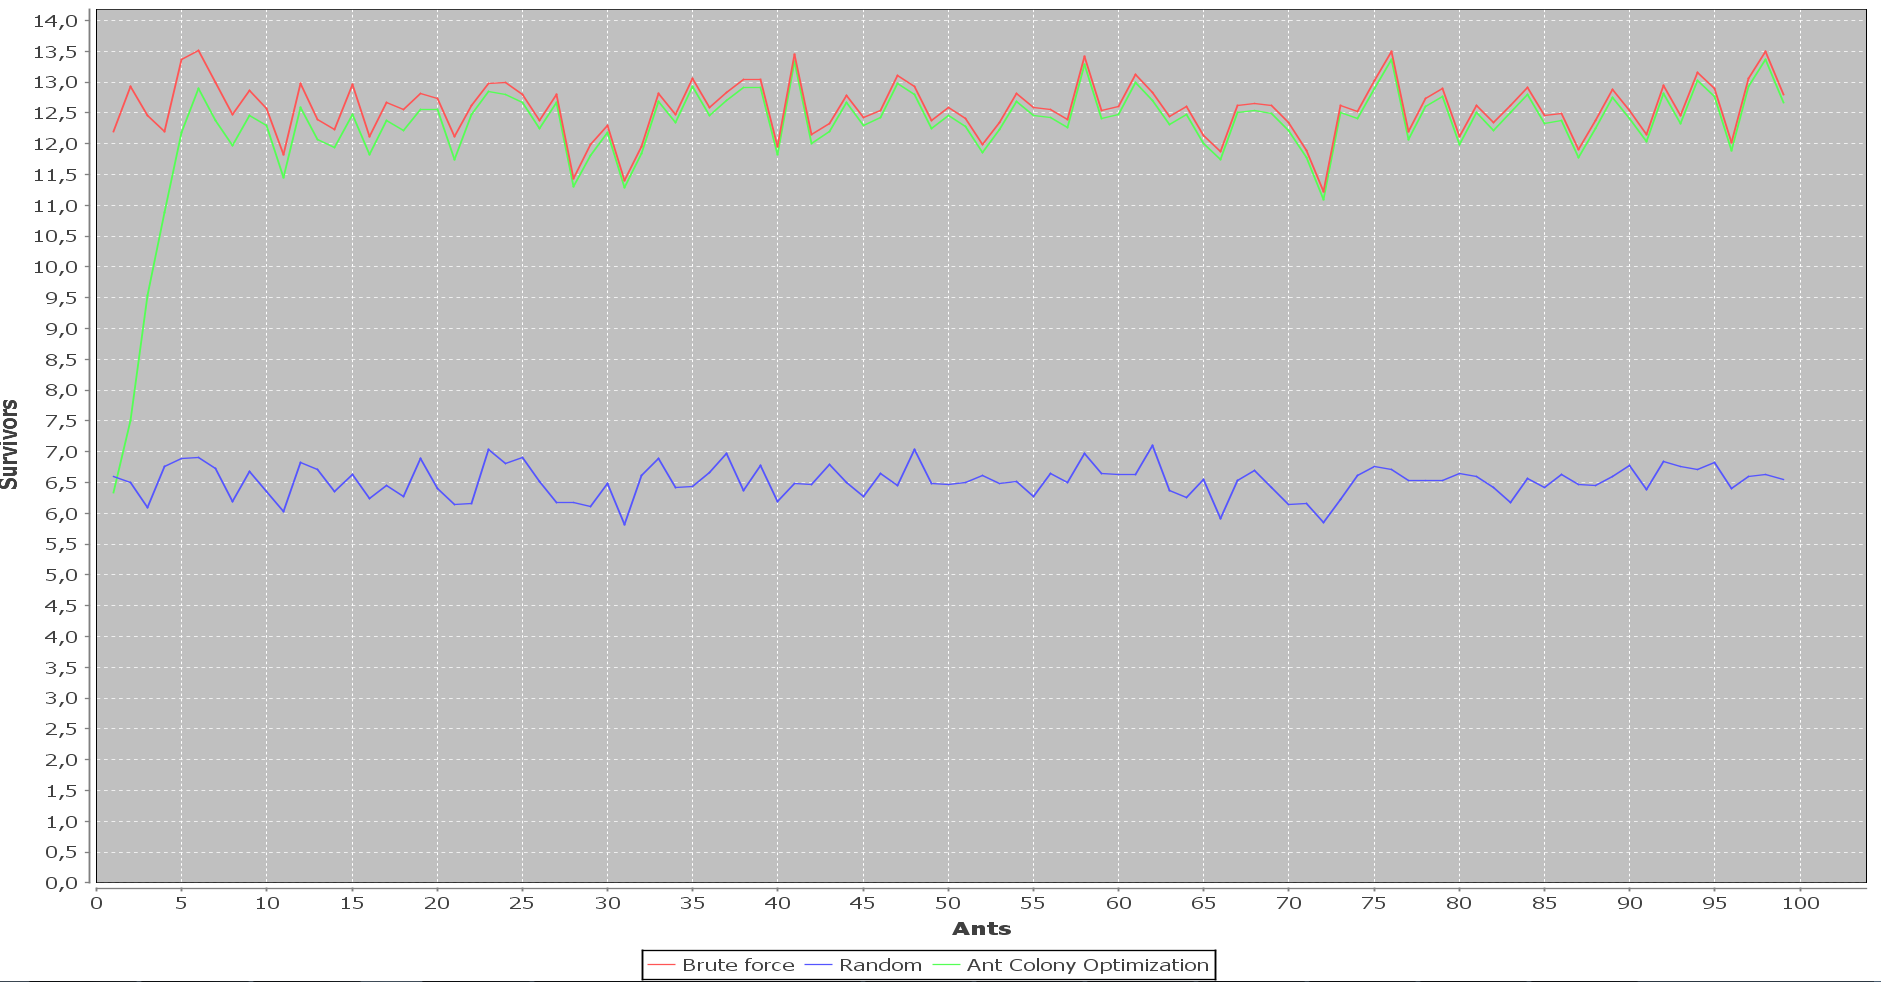
\includegraphics[width=150mm]{Float8Nodes2Leathal1Exitpng.png}
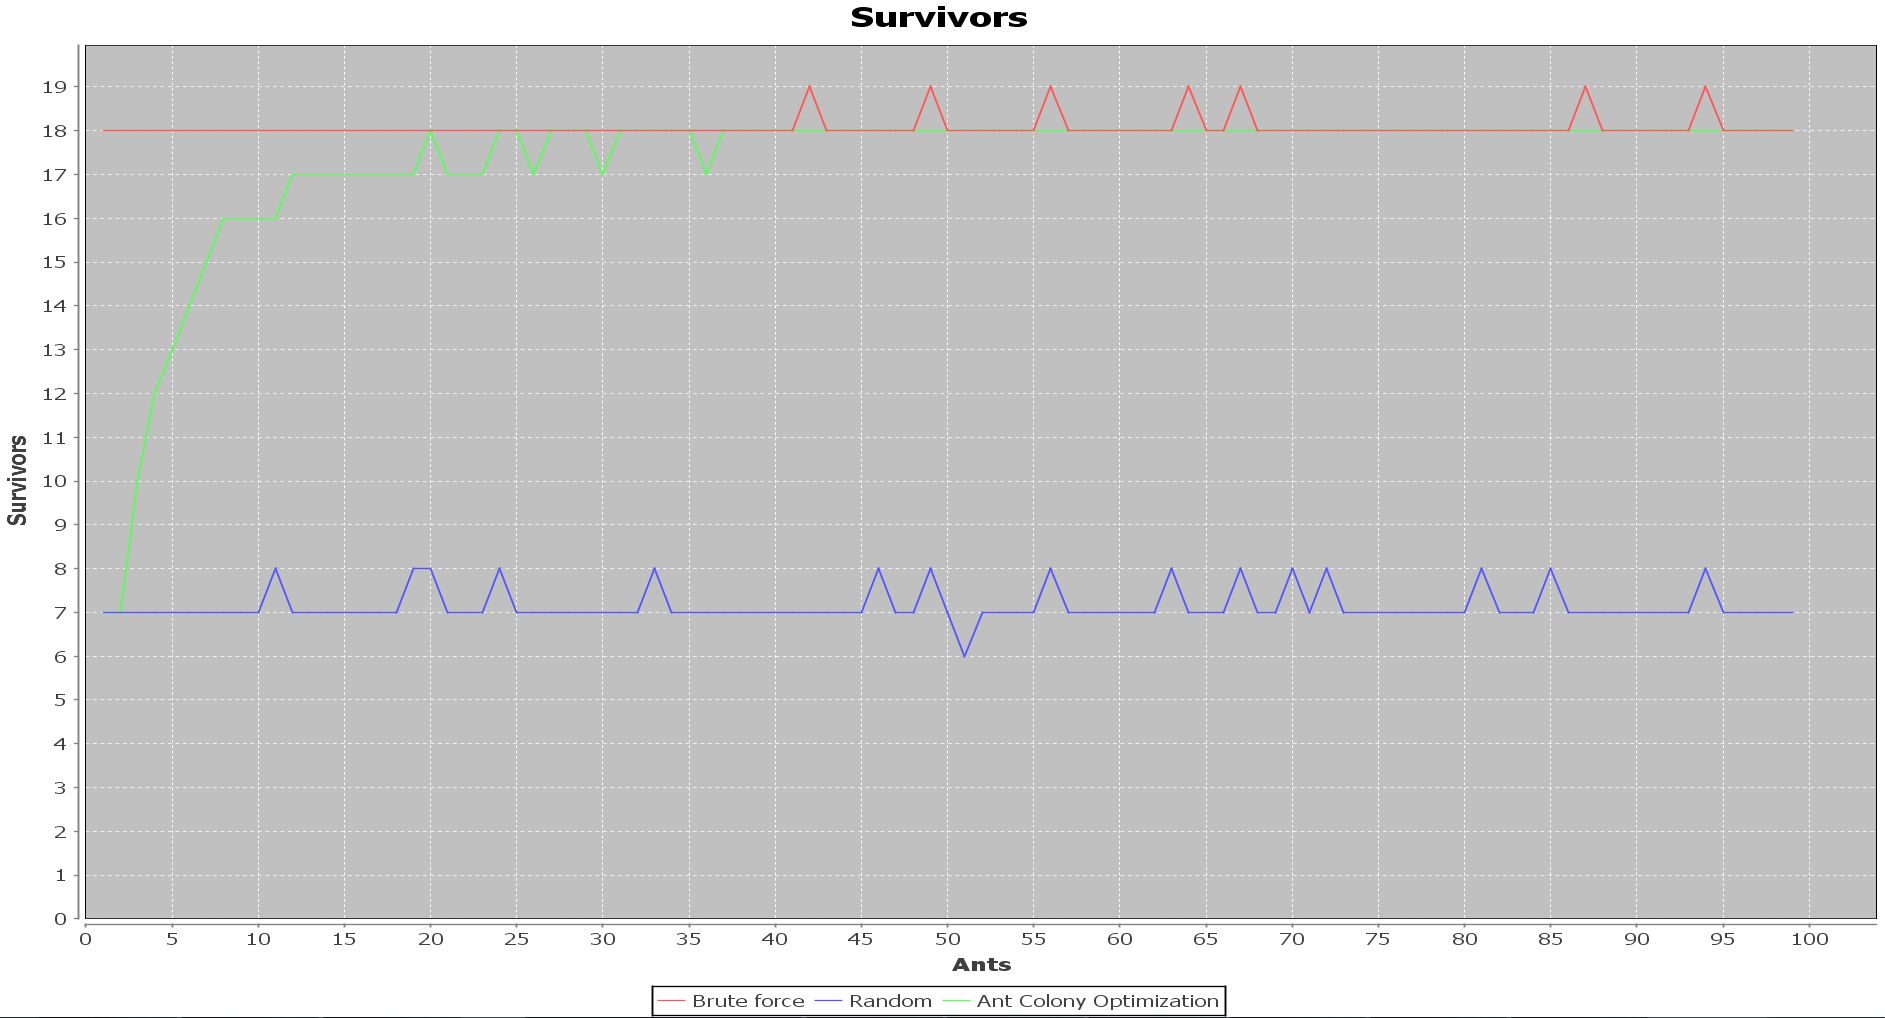
\includegraphics[width=150mm]{40Nodes2Leathal2Exit.png}